% Modelo de slides para projetos de disciplinas do Abel
\documentclass[aspectratio=169,11pt,handout]{beamer}

\usetheme[%
 sectionpage=none,%
 subsectionpage=progressbar%
 ]{metropolis}
\useoutertheme{infolines}
\setbeamersize{text margin left=1cm,text margin right=1cm}
\setbeamertemplate{part page}
{
  \begin{centering}
    \begin{beamercolorbox}[sep=16pt,center]{part title}
      \usebeamerfont{part title}\insertromanpartnumber.~\insertpart\par
    \end{beamercolorbox}
  \end{centering}
}

\usepackage[czech]{babel}
\usepackage{graphicx}
\usepackage{enumitem}
\usepackage{amsmath}
\usepackage{mathtools}
\usepackage{tcolorbox}

\tcbset{%
 sharp corners=all,%
 boxsep=7pt,%
 fonttitle=\bfseries,%
 colback=gray!30!white,%
 colframe=mDarkTeal,%
 boxrule=1pt%
}

\title{PSEUDOKÓD}
\date{\today}
\author{Adam Klepáč}
\institute[GEVO]{Gymnázium Evolution Jižní Město}

% enumerate global settings
\setlist[enumerate,1]{label=\arabic*.}
\setlist[enumerate,2]{label=\alph*)}
\setlist[itemize,1]{label=\textbullet}

\begin{document}

\maketitle

\part[Předmluva]{Předmluva}

\begin{frame}
 \partpage
\end{frame}

\begin{frame}
 \frametitle{Obsah}
 \tableofcontents
\end{frame}

\section[Program]{Počítačový program}
\subsection[CPU]{CPU}

\begin{frame}
 \frametitle{Co je CPU?}
 \begin{columns}
  \begin{column}{.3\textwidth}
   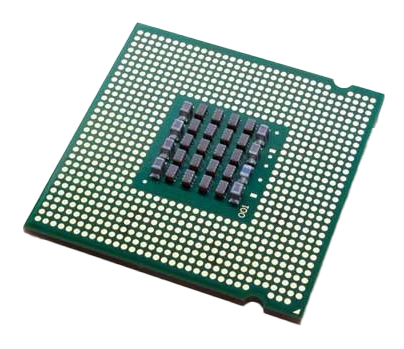
\includegraphics[width=\textwidth]{cpu}
  \end{column}
  \begin{column}{.7\textwidth}
   \begin{tcolorbox}
    CPU (\textbf{C}entral \textbf{P}rocessing \textbf{U}nit) je elektrický
    obvod, který vykonává \alert{instrukce} tvořící \alert{počítačový program}.
   \end{tcolorbox}
  \end{column}
 \end{columns}
\end{frame}

\subsection[Operace]{Operace}

\begin{frame}
 \frametitle{Fetch}
 \begin{tcolorbox}[title=Fetch,center,width=.95\textwidth]
  CPU \alert{vyzvedne} instrukci z programu.
 \end{tcolorbox}
 \begin{itemize}
  \item Instrukce je v programu uložena jako posloupnost nul a jedniček.
  \item Poloha (adresa) instrukce je dána čítačem (program counter). Postaru se
   mu někdy říká `hlava'.
  \item Čítač uchovává adresu poslední instrukce a po přečtení se posune o délku
   (v~bitech) zpracovávané instrukce.
 \end{itemize}
\end{frame}

\begin{frame}
 \frametitle{Decode}
 \begin{tcolorbox}[title=Decode,center,width=.95\textwidth]
  CPU \alert{přeloží} načtenou instrukci.
 \end{tcolorbox}
 \begin{itemize}
  \item Prvních pár bitů v instrukci obvykle značí operaci, která se má provést.
  \item Zbývající bity jsou pak například adresy operandů v paměti.
 \end{itemize}
\end{frame}

\begin{frame}
 \frametitle{Execute}
 \begin{tcolorbox}[title=Execute,center,width=.95\textwidth]
  CPU \alert{provede} přeloženou instrukci.
 \end{tcolorbox}
 \begin{itemize}
  \item V závislosti na architektuře CPU, instrukce obsahují buď jedinou akci
   nebo posloupnost akcí.
  \item Výsledek je uložen ve vnitřní paměti CPU. Uložení do vnější paměti
   (třeba RAM nebo disk) musí být obsahem nějaké další instrukce.
 \end{itemize}
\end{frame}

\subsection[Instrukce]{Typy instrukcí}

\begin{frame}
 \frametitle{Paměťové operace}
 \begin{itemize}
  \item<1-> \alert{SET}: Nastav blok vnitřní paměti na danou hodnotu.
  \item<2-> \alert{COPY}: Zkopíruj hodnotu z bloku vnitřní paměti do jiného bloku.
  \item<3-> \alert{READ/WRITE}: Zapisuj data nebo je čti z připojených zařízení.
 \end{itemize}
\end{frame}

\begin{frame}
 \frametitle{Početní a logické operace}
 \begin{itemize}
  \item<1-> \alert{Sečti/odečti/vynásob/vyděl} spolu hodnoty ve dvou blocích
   paměti.
  \item<2-> \alert{Konjunkce/disjunkce} dvou uložených hodnot.
  \item<3-> \alert{Porovnej} spolu dvě uložené hodnoty.
  \item<4-> Operace na desetinných číslech (\alert{floating point} arithmetic).
 \end{itemize}
\end{frame}

\begin{frame}
 \frametitle{Řídící (control flow) operace}
 \begin{itemize}
  \item<1-> \alert{Odboč} na jiné místo v programu a vykonej tamější instrukce.
  \item<2-> \alert{Podmínečně odboč} na jiné místo v programu a vykonej tamější
   instrukce.
  \item<3-> \alert{Zavolej} jiný blok kódu, uchovav následující instrukci jako
   místo návratu.
 \end{itemize}
\end{frame}

\part[Pseudokód]{Pseudokód}

\begin{frame}
 \partpage
\end{frame}

\begin{frame}
 \frametitle{Obsah}
 \tableofcontents
\end{frame}

\section[Definice a příklady]{Definice a příklady}
\subsection[Definice]{Definice}

\begin{frame}
 \begin{tcolorbox}[title=Pseudokód,center,width=.95\textwidth]
  Pseudokód je \alert{neformální} zápis počítačového programu/algoritmu.
 \end{tcolorbox}
\end{frame}

\subsection[Příklady]{Příklady}



\begin{frame}
 \centering\Huge Díky za pozorst.
\end{frame}

\end{document}
